\chapter{The simulator}

The purpose of the simulator is to visualize the movement of a simple snake robot model progressing according to a predefined path and obstacles in the environment.

This chapter aims at describing how the simulator is structured and can be used, as well as explaining particular code snippets in more detail. Moreover, it provides an overview of how the mathematical background is applied.

%-----------------------------------------------------------------------------------
%-----------------------------------------------------------------------------------

\section{System flow}

  The system flow is illustrated in figure \ref{fig:prog_flow}. Initialization is performed based on the given snake robot and obstacle configurations. Furthermore, the joint acceleration $\mathbf{\ddot{q}}$ of the robot is found by solving the dynamics equation (\ref{eq:eom_qdd}), where the joint torque $\boldsymbol{\tau}$ is calculated by the computed torque control. The control reference is based on deviation from the desired trajectory. Joint velocities $\mathbf{\dot{q}}$ and angles $\mathbf{q}$ are deduced from $\mathbf{\ddot{q}}$ using Euler integration.

Whenever the robot is in contact with one or more obstacles, the joint velocities are projected onto the allowable position space using the intersect of all $\prescript{j}{ap}{P}$, explained in \ref{subseq:HPFC}.

\begin{figure}
    \centering
    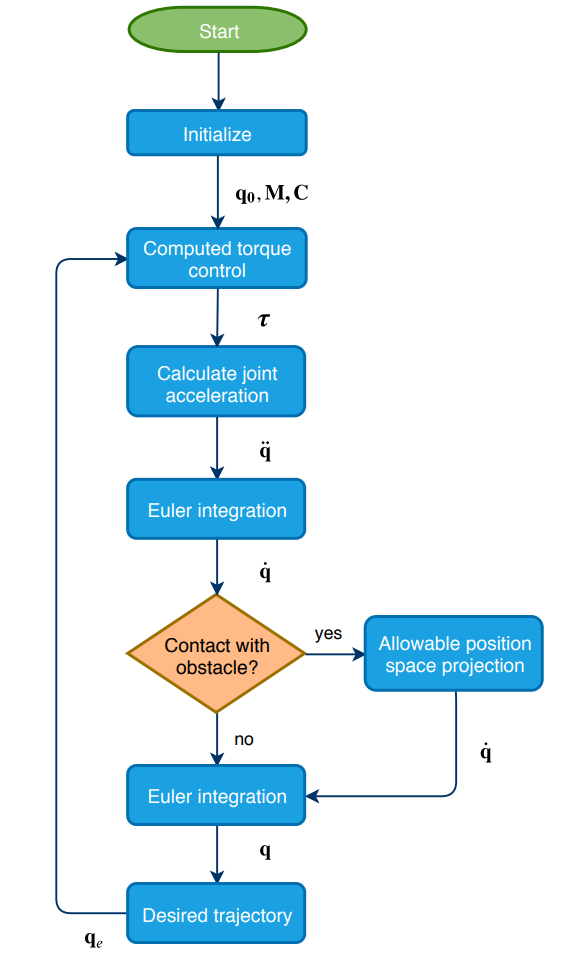
\includegraphics[width=0.7\textwidth]{figures/sysflow.PNG}
    \caption{Program flow diagram}
    \label{fig:prog_flow}
\end{figure}



%-----------------------------------------------------------------------------------
%-----------------------------------------------------------------------------------

\section{Simplifications}

Expressing the complete dynamics of the system includes explicitly finding the part of the joint torques that are not directly applied to the robot joints, but rather as a force acting on the external obstacles. In other words, the torque would have to be separated in a component belonging to the constraint- or propulsion space and a component that belongs to the shape space (see \ref{subseq:snakeHPFC}). \hl{Could we have used Paf to find the component belonging to the constraint++ space???????}

This challenge combined with a strict time schedule has led to a simplification in the development of the simulator. In the simulator, the movement of the robot is first calculated under the assumption that no obstacle is present. To account for this, the interaction forces are implicitly considered through mapping to the allowable position space. This means that if the robot is in contact with the environment, the joint velocities are influenced accordingly.

\hl{Discretization.}


%En mulighet er å finne bevegelsesligningene for constrained motion som Yukomannen, men han har abstrahert seg bort fra en del av de kontaktkreftene så de må beregnes eksplisitt. Constraint bev-ligningene er i stand til å forklare den bevegelsen man faktisk får. Begge bev.lignningene gjelder, det er bare at Yukomannen har abstrahert seg bort fra kontaktkreftene ved å si at den bevegelsen kan ikke gå dit men dit. Men det som aksellererer (kreftene) er ikke eksplisitt uttrykt. De er kun uttrykkt med en q prikk prikk pluss C q prikk. Det er litt som kreftene mellom leddene i roboten. Det er krefter der og vi definerer dem aldri eksplisitt (fordi de deltar ikke i energiproduksjon), men de er jo implisitt med i modellen til alle tider. Litt samme jeg har gjort - gått bort fra eksplisitt forhold til kreftene fordi føringskreftene er gitt av kinematikken (et sett med constraints)

%Har tatt et valg om å gjøre det på en annen måte. Tidspress. Går ut i fra en bev.ligning som går ut i fra ingen constraints. Og M og C merker ikke constraints fordi vi ikke måler q osv.

%This challenge has led to a simplification in the development of the simulator. Instead of explicitly including the external force in the dynamics, the movement of the robot is simulated for one time step under the assumption that no obstacle is present. The resulting joint velocities are then projected onto the allowable position space restricted by the obstacles. The time step of impact between the bodies is thus skipped.

\section{Restrictions/Limitations}

\section{User guide}

The user can adjust parameters related to the specifications of the snake robot, obstacles in the environment, the desired path the robot should attempt to follow and control parameters. Once the variables are adjusted in the respective files, the \texttt{initialization.m} script can be run. For a specific configuration, this initialization only has to be run once for every time MATLAB is started. The variables will then end up in the MATLAB workspace and the simulation can be run for a wished number of times. Variables that do not change the dynamics of the robot can be redefined without running the whole initialization over.

The user definable variables are summarized in table \ref{tab:sim_userparams}.

\begin{table}
\centering
    \begin{sideways}
    \begin{tabular}{|c|c|c|c|c|}
        \hline
        \textbf{\small{Parameter description}} & \textbf{\small{Parameter name}} & \textbf{\small{Filename}} & \textbf{\small{Datatype}} & \textbf{\small{Unit}}\\
        \hline \hline
        \footnotesize{Number of links} & \texttt{n} & \texttt{init\char`_snake.m} & Integer & \\
        \hline
        \footnotesize{Link length} & \texttt{l}  & \texttt{init\char`_snake.m} & Float & $m$\\
        \hline
        \footnotesize{Link mass} & \texttt{m} & \texttt{init\char`_snake.m} & Float & $kg$\\
        \hline
        \footnotesize{Initial robot configuration} & \texttt{q0} & \texttt{init\char`_snake.m} & Array of floats & $rad$\\
        \hline
        \footnotesize{Number of obstacles} & \texttt{num\char`_obstacles} & \texttt{init\char`_obstacles.m} & Integer & \\
        \hline
        \footnotesize{Obstacle coordinates} & \texttt{obstacle\char`_coords} & \texttt{init\char`_obstacles.m} & 2D array of floats & $m$\\
        \hline
        \footnotesize{Obstacle safety radius} & \texttt{obstacle\char`_radius} & \texttt{init\char`_obstacles.m} & Float & $m$\\
        \hline
        \footnotesize{Proportional control gain} & \texttt{kp} & \texttt{init\char`_control.m} & Float &\\
        \hline
        \footnotesize{Derivative control gain} & \texttt{kd} & \texttt{init\char`_control.m} & Float &\\
        \hline
        \footnotesize{Torque saturation limit} & \texttt{max\char`_tau} & \texttt{init\char`_control.m} & Float & $Nm$\\
        \hline
    \end{tabular}
    \end{sideways}
    \caption{User adjustable simulator parameters}
    \label{tab:sim_userparams}
\end{table} 

\hl{Hvordan justere selve visualiseringen}
\hl{Hvordan endre desired path.}
\hl{Hvordan ser roboten osv ut}

\section{Program code summary}

The whole simulator is made, and to be executed, in MATLAB. The symbolic math toolbox has been used to generalize the code and make it adaptable to an n-link snake robot. The whole code can be accessed through ...

The constants $l$, $m$, $n$, $N$, $K_p$, $K_d$ from chapter \ref{chapter:theory}, as well as symbols for $\mathbf{q}$ and $\mathbf{\dot{q}}$ are globally defined and accessible for scripts/functions that might need them.

\subsection{Dynamics functions}

The dynamics, more particularly the matrices $M$ and $C$ from (\ref{eq:eom}), are generated symbolically in the script \texttt{init\char`_dynamics.m}.
As a result of the use of symbols, the matrices can be used as functions with the joint angles and velocities as input parameters.


\subsection{Kinematics functions}\label{subseq:kinfunc}

The script \texttt{init\char`_kinematics.m} generates the transformation matrices from the base to every link endpoint. These matrices are, equivalent to the dynamic matrices from last section, expressed with symbols. Additionally, functions for generating the rotation matrix around the z-axis, \texttt{Rz\char`_func(theta)}, and translation matrix in the x- and y direction, \texttt{D\char`_func(x\char`_dist, y\char`_dist)} are defined.

%-----------------------------------------------------------------------------------------
%-----------------------------------------------------------------------------------------

\subsection{Contact Jacobian function}
The symbolic expression of the contact Jacobians are calculated in\\ \texttt{init\char`_contact\char`_jacobians.m}. As there can be a maximum of one obstacle touching each link, there is one contact Jacobian calculated per link. The position of the contact point in world coordinates expressed by the joint variables is extracted from the homogeneous transformation matrix (see \ref{sec:kin}) on lines 2-9. The variable \texttt{q} represents the vector of generalized coordinates. The functions  Lines 11-14 perform partial differentiation of the position with respect to the generalized coordinates to obtain the contact Jacobian. All contact Jacobians are stacked in a 3-dimensional matrix on line 16. \texttt{Rz\char`_func(theta)} and \texttt{D\char`_func(x\char`_dist, y\char`_dist)} are previously defined functions, see \ref{subseq:kinfunc}.

\lstinputlisting[firstline=23, lastline=39]{Simulator_code/init_contact_jacobians.m}

%-----------------------------------------------------------------------------------------
%-----------------------------------------------------------------------------------------

\subsection{Projection function}

The projections are calculated in the function \texttt{calc\char`_projections.m} based on the functions for the contact Jacobians. 

In the following code snippet from the function, contact on the link \texttt{i} is established and the corresponding projection matrices are found. \texttt{q(n+2+i,k)} corresponds to the generalized coordinate $d_{c,i}$ (see section \ref{seq:constr_kin} for the vector of generalized coordinates).

\lstinputlisting[firstline=72, lastline=82]{Simulator_code/calc_projections2.m}

Seeing as there might be more than one contact point, several projection matrices are calculated. These matrices are combined by taking the union and intersect as described in \ref{subseq:HPFC}. The logic of the union- and intersect functions are borrowed from Øyvind Stavdahl and presented below.

\lstinputlisting[firstline=91, lastline=99]{Simulator_code/calc_projections2.m}

%-----------------------------------------------------------------------------------------
%-----------------------------------------------------------------------------------------

\subsection{Control}
The following function calculates the joint torques from the computed torque control scheme in \ref{subsec:comp_torque}. The saturation is based on the user-adjustable parameter \texttt{max\char`_tau}.

\lstinputlisting[]{Simulator_code/computed_torque_control.m}

\subsection{Visualization}

The robot simulation is performed by displaying a figure which is redrawn for every time step based on the given robot and obstacle data. The function in \texttt{visualize.m} takes care of this.

